% !TeX spellcheck = en_US
% !TeX encoding = UTF-8
% !TeX root = ../report.tex

\chapter{Method}
\label{chp:Method}

\section{V-Disparity}

This chapter explains the theoretical basis of the V-disparity method. To begin with, the basis of the V-Disparity method, the disparity map, is outlined.

\subsection{Disparity Map} \label{sbs:method_dispmap}
It is assumed, that the reader has a general understanding of stereovision systems. Given two calibrated stereo cameras, the respective rectified images can be used to calibrate a disparity for each pixel. These is achieved with different block-matching algorithms, such as the StereoSGBM algorithm implemented in the popular OpenCV library. Given a disparity map, the baseline and focal length, a depth map can be calculated and used for further processing. The V-Disparity method however only makes use of the disparity map.


%Elaborate on calculation and formulas of disparity

\subsection{V-Disparity}

Once a disparity map $\Delta$(u,v) was computed, a V-Disparity histogram can be constructed. For each row u, a histogram of the occuring disparities in this row is computed. The histogram values represent the occurence of the respective disparity in the row, where each bin is represented by a pixel. Given a plane in a scene, the projection of the plane onto the V-Disparity image has a useful property. 
A plane will be projected as a linear curve in the V-Disparity image. This simplifies the extraction of the respective plane in the V-Disparity image, as a e.g. Hough Line Transform can be applied to detect the lines. Consequently, the detection of straight lines in the V-Disparity corresponds to detection of planes in the scene.
A scene is therefore made up of planes, where vertical planes can be understood as obstacles, horizontal planes as the road when flat, or as a set of oblique planes when the road is non-flat. Hu et al. \cite{Hu2005} offer an in-depth analysis of the projection of the three above types of planes.

\newline

Because the most prominent plane in usually represented by the ground, it will be detected as the line with the most votes in the V-Disparity image. Horizontal or vertical lines can be dismissed, as the disparity gradient of the road leads to a skewed line.
Horizontal lines can be associated with obstacles and used for obstacle detection.
Even though Non-flat road geometry will not be considered in this project, it should be noted that the road in that case can be approximated by a series of planes, which will then be projected as a piecewise linear curve in the V-Disparity image.

Once the line has been fitted in the V-Disparity image, the disparity values for the road surface are known. Extracting the road in the image domain is straightforward. For each row, the values which lie within a threshold of the value of the extracted line are part of the road, all other pixels are masked as non-road.

\begin{figure}
	\centering
	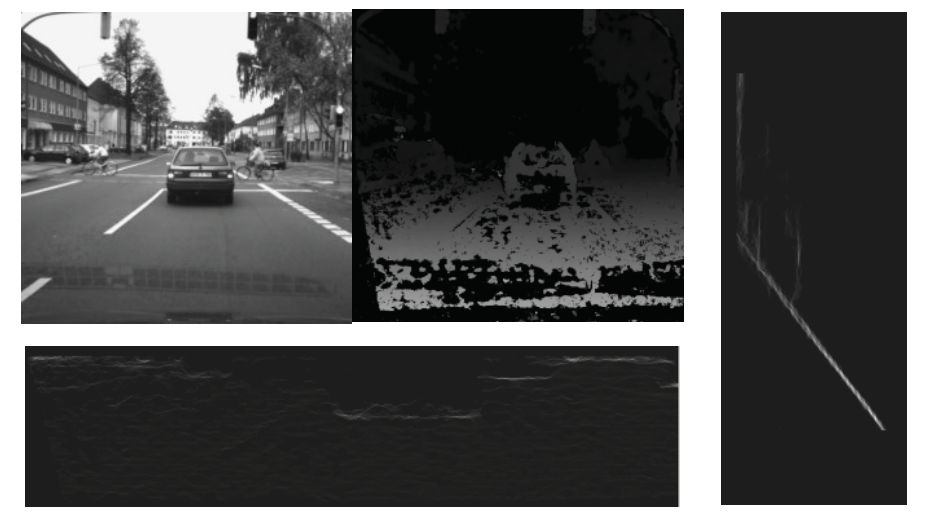
\includegraphics[width=0.7\linewidth]{Figures/vdisp}
	\caption[Overview of V-Disparity method]{}
	\label{fig:vdisp}
\end{figure}

Oniga et al. \cite{Oniga2015} show a camera image, the corresponding dispartiy map and the V- and U-Disparity respectively.



\section{Lidar Camera Projection}

To project lidar scanning points onto a camera image, the camera's intrinsic parameters should be known. Additionally, the projection matrix from lidar to camera should needs to be determined. It can be measured by hand and computed, or determined by externally calibrating the lidar and camera with an automated pipeline.
\newline
After driving a few laps on our indoor Gokart track, the lidar generates an occupancy grid. This occupancy grid is then projected onto the camera frame. By determining the relative pose and orientation of the camera with respect to the world frame, one can then project all points corresponding to the road onto the camera frame.